\part{Comparison} \label{part:Comparison and implementation}

\chapter{comparisons and implementations}

This chapter will analyze the characteristics of the three algorithms on different real-world data sets. Taking into account the differences between instances (N) and dimension (M), 6 data sets with different N and M will be tested. The code will test the AUC values of the algorithms, and first analyze the individual variables. Then, analyze the variables that affect each other according to the generated heatmap. Finally, this work will take 5 representative values from each variable of each algorithm, use grid search algorithm to find the parameters that each algorithm performs best on the same data set. Analyze the performance difference of $R_{NX}$ curve.\\

\noindent As discussed above, in order to draw the conclusions in a convincing way, This work will examine the three algorithms' quality on several real-world data sets with different N and M, base on the neighborhood-based DR performance criteria discussed above. there are six public databases: Iris, Wine, Breast Cancer Wisconsin Diagnostic (BCW), Optical Recognition of Handwritten Digits test set (Digits), the Olivetti faces (Oliv) and Labeled Faces in the Wild face recognition(LFW).\\

\begin{center}
\begin{tabular}{|c|c|c|}% 通过添加 | 来表示是否需要绘制竖线
\hline  % 在表格最上方绘制横线
Datasets & Number of instances & Number of dimensions\\
\hline  %在第一行和第二行之间绘制横线
Iris & 150 & 4\\
\hline  %在第一行和第二行之间绘制横线
Wine & 178 & 13\\
\hline  %在第一行和第二行之间绘制横线
BCW & 569 & 30\\
\hline  %在第一行和第二行之间绘制横线
Oliv & 400 & 4096\\
\hline  %在第一行和第二行之间绘制横线
Digits & 1797 & 64\\
\hline  %在第一行和第二行之间绘制横线
LFW & 13233 & 5749\\
\hline % 在表格最下方绘制横线
\end{tabular}\\
\end{center}
\\

\noindent When we are analyzing the result, we should consider that the high-dimensional sphere was modeled by probability graph, the t-SNE algorithm adapts its "distance" concept to changes in regional density in the data set. As a result, it naturally expands dense clusters and shrinks sparse clusters, making the clusters roughly uniform in size. It also makes it difficult to see the relative size of clusters in the t-SNE graph, and the distance between clusters in low dimensions does not represent the distance between clusters in high dimensions.

\section{Grid search algorithm}

Grid search is a parameter adjustment method, with exhaustive strategy: among all the predetermined parameter selections, through looping and trying every possibility, the best performing parameter is the final result. The principle is only in one part. Take this thesis's work as an example. Each algorithm selects the four most important parameters, and each parameter takes 5 typical values. All possibilities are listed, which can be expressed as a 5*5*5*5 four-dimensional table. Each numerical combination is a grid, and the cycle process is like traversing and searching in each grid, so it is called grid search. As for this work, the code will go though all combination of parameters and return the best parameters considering neighborhood-based DR performance criteria.

\section{t-SNE}
There are 4 most important parameters for t-SNE, the ideas of each parameters are: 

\begin{enumerate}[1)]
\item $perplexity$: number of nearest neighbors for each point
\item $n\_iter$: maximum number of iterations for optimization
\item $early\_exaggeration$: the tightness inside clusters and the distance inbetween
\item $min\_grad\_norm$: the threshold for stopping the optimization 
\end{enumerate}\\



\subsection{$perplexity$}

\noindent $perplexity$ represent the number of neighbors each point t-SNE considers. It explains how to maintain a balance between the local and global aspects of the data. The perplexity value has a complex effect on the generated pictures, but the performance of SNE is quite reliable for changes in complexity, and the typical value of perplexity is between 5 and 50\cite{ref9}. Also, since the perplexity means the number of the neighbors, it should not be higher than the number of data points.\\

\noindent We can try different potential perplexity values in datasets with different instances. At the same time, since the algorithm using stochastic method, the parameter $random\_state$ is set to 1. This parameter determines the random number generator so that it pass an int mark for reproducible results across multiple function calls. After examining it on the first dataset Iris, we get the figures below:

\begin{figure}[H]
\centering  %图片全局居中
% \subfigure[name1]
{
\label{Fig.sub.1}
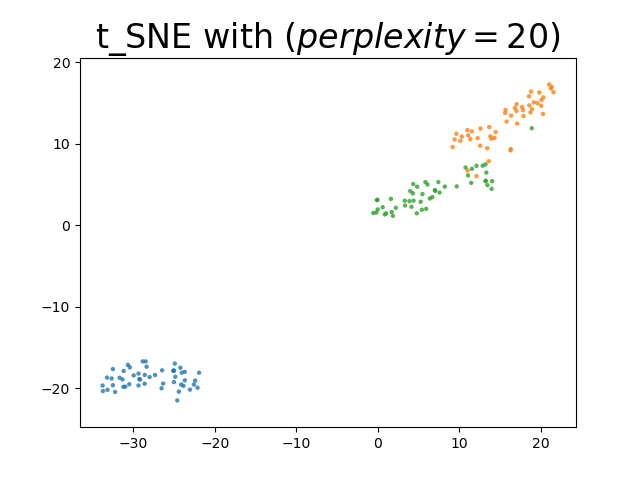
\includegraphics[width=7cm,height=3.5cm\textwidth]{images/image_comparison_tsne_perp20.png}}
% \subfigure[name2]
{
\label{Fig.sub.2}
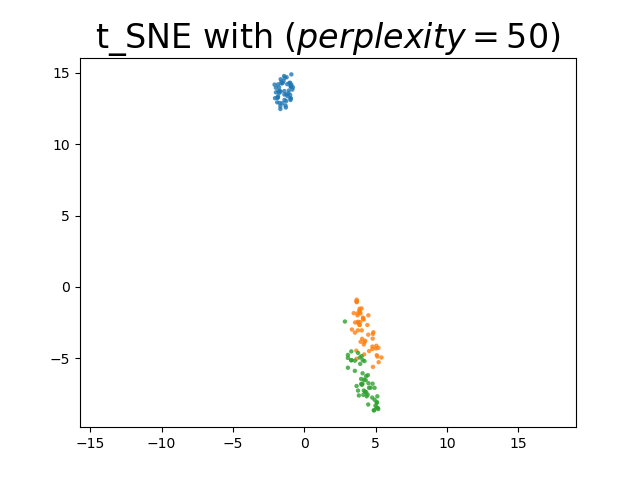
\includegraphics[width=7cm,height=3.5cm\textwidth]{images/image_comparison_tsne_perp50.png}}
\caption{LD result for t-SNE with perplecity 20 and 50}
% \label{LD result for t-SNE with n_iter 300 and 500}
\end{figure}

\begin{figure}[H]
\centering  %图片全局居中
% \subfigure[name1]
{
\label{Fig.sub.1}
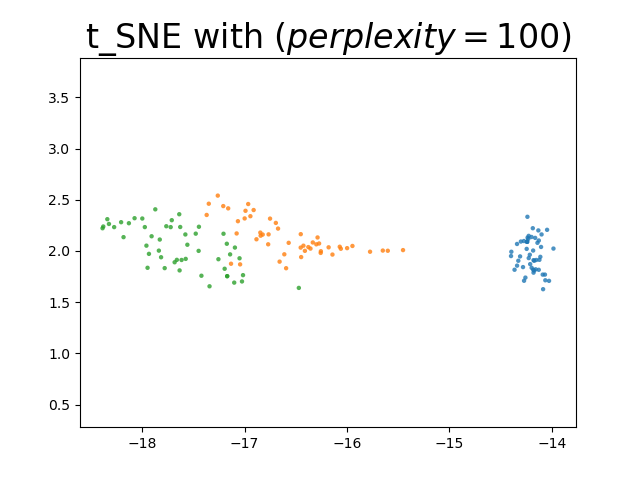
\includegraphics[width=7cm,height=3.5cm\textwidth]{images/image_comparison_tsne_perp100.png}}
% \subfigure[name2]
{
\label{Fig.sub.2}
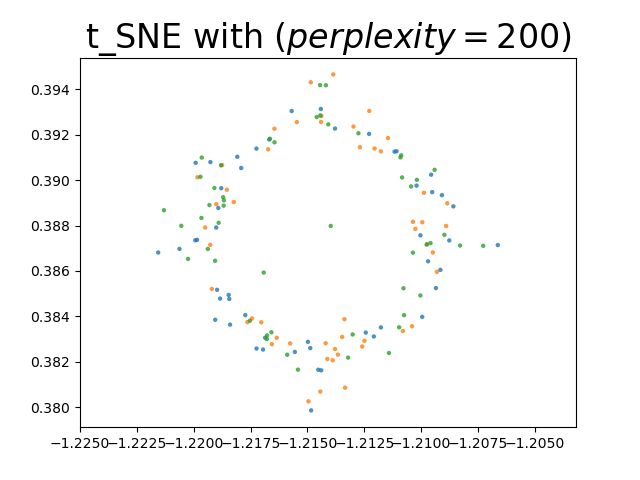
\includegraphics[width=7cm,height=3.5cm\textwidth]{images/image_comparison_tsne_perp200.png}}
\caption{LD result for t-SNE with  perplecity 100 and 200}
% \label{Fig.main}
\end{figure}


\noindent In the figure, we can see that when the value is in the range of 5-50, clusters are well distinguished. Considering that the number of instances of the dataset is only 150, when the value is 100, the clusters begin to merge. When the perplexity = 200, it is difficult to distinguish different clusters. In order for the algorithm to work properly, the perplexity should actually be less than the number of points. Considering the experimental results and the strategy of the search about the optimal number of neighbor from K nearest neighbour algorithm\cite{ref12}, we can simply set perplexity to $n^{0.5}$, where n stand for number of instances. \\

\noindent At the same time, the $AUC$ value for the result with these parameters are 0.731, 0.658, 0.654, -0.004 separately. These $AUC$ values verifies the previous observations. As for the last one, it has a big difference between others and also the only minus result. With the definition of the $R_{NX}$ curve $R_{NX} (K) = ((N − 1)Q_{NX} (K) − K) /(N − 1 − K)$, this is because the K is higher than N in the formula. Numerator is relative small and denominator is a negative number, we then have a minus result.

\subsection{$min\_grad\_norm$}

This parameter is the threshold of gradient norm to determine when the optimization will be stopped. If the norm is less than the setting value, the gradient descent of Kullback-Leiber divergence will stop.

\subsection{$n\_iter$}

\noindent $n\_iter$ is the maximum number of iterations for the algorithm. The graph observed above are all generated with 1000 iteration which is the default value of $n\_iter$. In principle, the higher $n\_iter$ gives the better result. However, it may be very time consuming when it comes to big dataset. In contrast, if $n\_iter$ is too small, the algorithm does not have enough iteration to generate the convincing clusters in LD. The most important thing is to reach a stable configuration. The figure shows how the result changes with $n\_iter$ grows in Digits dataset as above:

\begin{figure}[H]
\centering  %图片全局居中
% \subfigure[name1]
{
\label{Fig.sub.1}
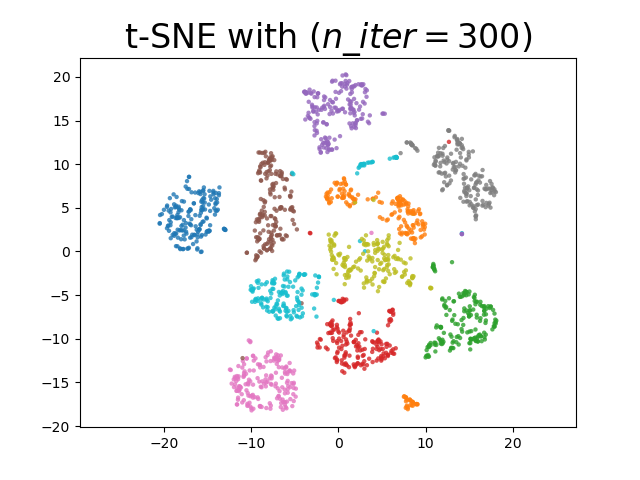
\includegraphics[width=7cm,height=3.5cm\textwidth]{images/t-sne/tsne_niter_300.png}}
% \subfigure[name2]
{
\label{Fig.sub.2}
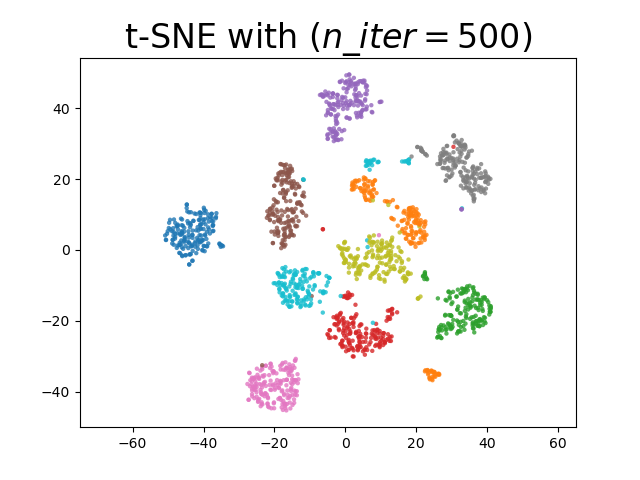
\includegraphics[width=7cm,height=3.5cm\textwidth]{images/t-sne/tsne_niter_500.png}}
\caption{LD result for t-SNE with n\_iter 300 and 500}
% \label{Fig.main}
\end{figure}

\begin{figure}[H]
\centering  %图片全局居中
% \subfigure[name1]
{
\label{Fig.sub.1}
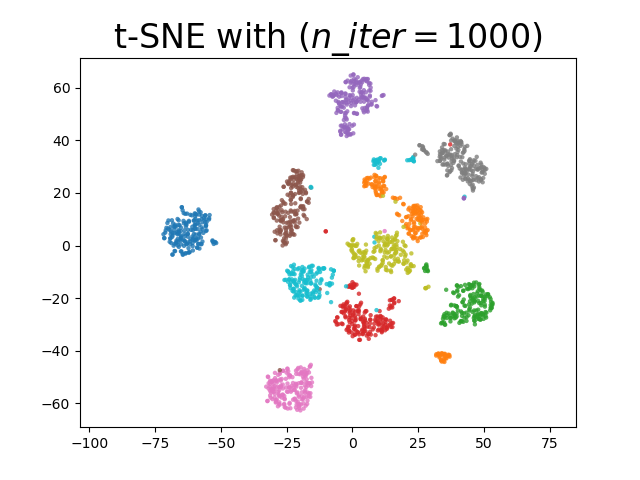
\includegraphics[width=7cm,height=3.5cm\textwidth]{images/t-sne/tsne_niter_1000.png}}
% \subfigure[name2]
{
\label{Fig.sub.2}
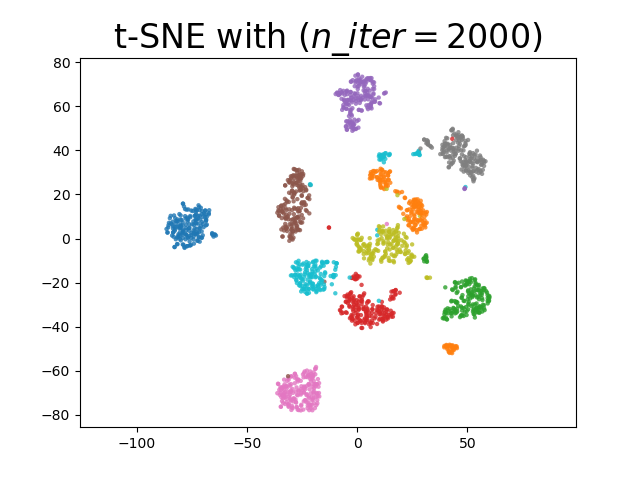
\includegraphics[width=7cm,height=3.5cm\textwidth]{images/t-sne/tsne_niter_2000.png}}
\caption{LD result for t-SNE with n\_iter 1000 and 2000}
% \label{Fig.main}
\end{figure}

\noindent From the figure, we can easily observe that the more iterations, the more well identified for clusters. These four $n\_iter$ generate $AUC$ values for 0.489, 0.526, 0.533, 0.536 separately, which verified the previous conclusion.


\subsection{$early\_exaggeration$}

$ early\ _exaggeration $ is a technique in which all $p_{ij}$ are multiplied and "exaggerated" in the early stages of optimization by multipling all $p_{ij}$s a fixed number in the initial stages of the optimization. This means that almost all of the $q_{ij}$ ’s, which still add up to 1, are much too small to model their corresponding $p_{ij}$ ’s. The result of this is to force the value of $q_ {ij}$ to be more concentrated on the larger $ p_{ij} $s, especially for closer points, thereby making the earlier clusters more tightly bound together This creates a lot of relatively empty space in the map, which makes it much easier for the clusters to move around relative to one another in order to find a good global organization\cite{ref13}. By doing that, it can control the closeness of clusters in high-dimensional space and the distance between them in low-dimensional space. For larger values, the space between natural clusters will be larger in the embedded space.


\subsection{Relations between parameters}

The algorithm also generates a series of heatmaps to show the relationship of each parameter pair. The algorithm also generates a series of heatmaps to show the relationship of each parameter pair. Heatmap represents the effect of one parameter change on another parameter when other parameters take default values. According to the operation of t-SNE on 6 data sets, there are several interesting findings worth showing:

\subsubsection{$early\_exaggeration$ and $n\_iter$:}
\subsubsection{$early\_exaggeration$ and $perplexity$:}
\subsubsection{$perplexity$ and $n\_iter$:}

\subsubsection{Running time:}

As in the previous theoretical analysis,  It is easy to find that running time increase with $perplexity$ and $n\_iter$ affect the running time the most. The time increases significantly with these two variables independently with the same trend on 6 data sets. Take digits as an example, there are heatmaps for time:

\begin{figure}[H]
\centering  %图片全局居中
% \subfigure[name1]
{
\label{Fig.sub.1}
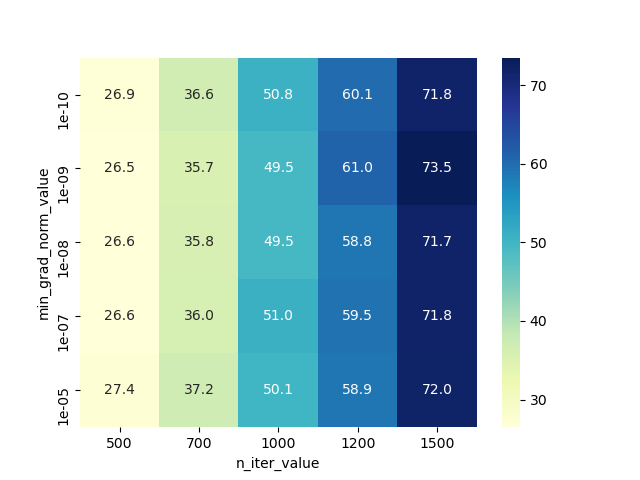
\includegraphics[width=4.5cm,height=4.5cm\textwidth]{images/t-sne/Digit_elapsed_time_min_grad_norm_value_n_iter_value_heatmap.png}}
% \subfigure[name2]
{
\label{Fig.sub.2}
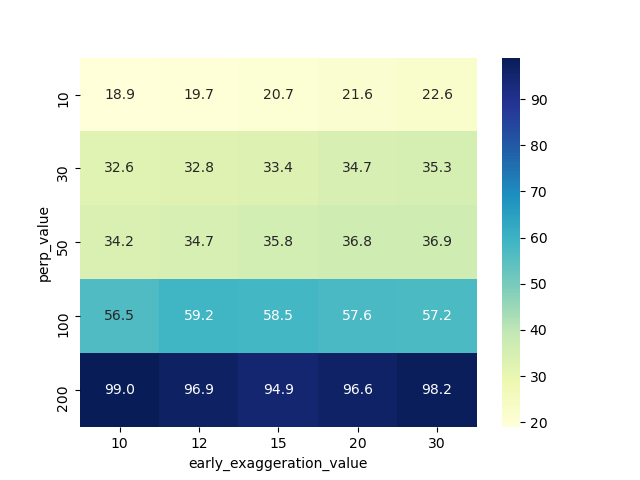
\includegraphics[width=4.5cm,height=4.5cm\textwidth]{images/t-sne/Digit_elapsed_time_perp_value_early_exaggeration_value_heatmap.png}}
{
\label{Fig.sub.3}
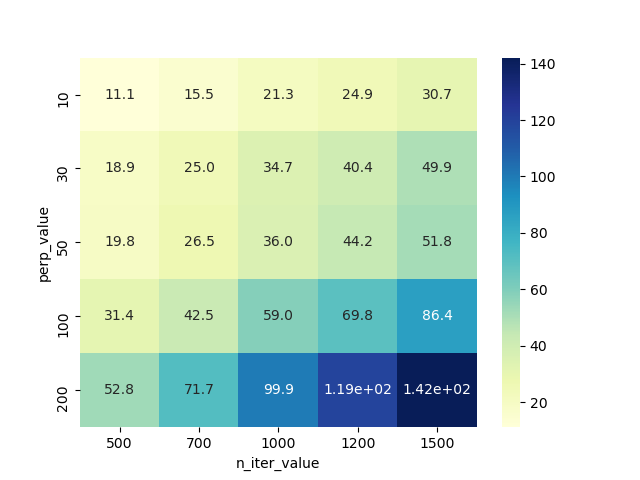
\includegraphics[width=4.5cm,height=4.5cm\textwidth]{images/t-sne/Digit_elapsed_time_perp_value_n_iter_value_heatmap.png}}
\centering
\caption{Running time for perplexity and n\_iter with other parameters and with each other }
% \label{Fig.main}
\end{figure}

\section{UMAP}
There are 4 most important parameters for UMAP, the ideas of each parameters are:

\begin{enumerate}[1)]
\item $n_neighbors$: The size of local neighborhood like perplexity for t-SNE
\item $spread$: The effective scale of embedded points
\item $min\_dist$: The effective minimum distance between embedded points.
\item $negative\_sample\_rate$: Number of negative samples for per positive sample
\end{enumerate}\\

\subsection{$n\_neighbors$}

The size of the local neighborhood used for manifold approximation. This parameter controls how UMAP balances local versus global structure in the data. It does this by constraining the size of the local neighborhood UMAP will look at when attempting to learn the manifold structure of the data. This means that low values of $n\_neighbors$ will force UMAP to concentrate on very local structure (potentially to the detriment of the big picture), while large values will push UMAP to look at larger neighborhoods of each point when estimating the manifold structure of the data, losing fine detail structure for the sake of getting the broader of the data. Also, since the $n\_neighbors$ means the number of the neighbors, it should not be higher than the number of data points.\\

\noindent We can try different potential perplexity values in datasets with different instances.With the same time as t-SNE, in order to avoid the effect of stochastic for each round, the parameter $random_stateis$ set to 1. After examining it on the dataset Digits, we get the figures below:

\begin{figure}[H]
\centering  %图片全局居中
% \subfigure[name1]
{
\label{Fig.sub.1}
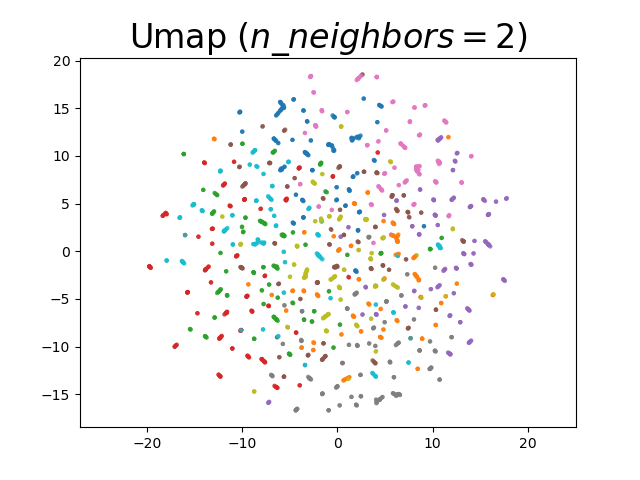
\includegraphics[width=7cm,height=3.5cm\textwidth]{images/umap/umap_digit_n_neighbor_2.png}}
% \subfigure[name2]
{
\label{Fig.sub.2}
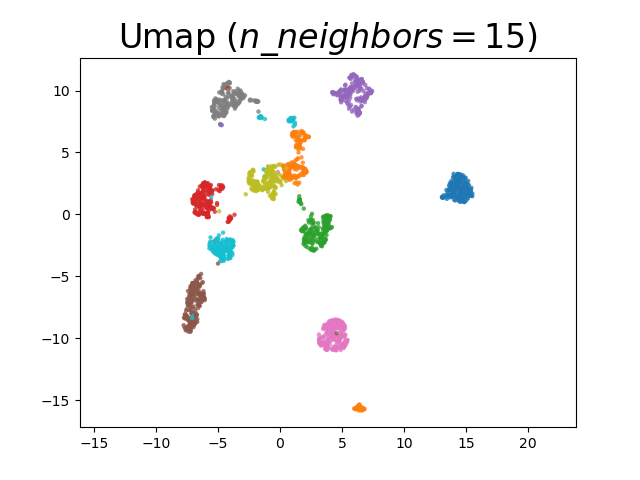
\includegraphics[width=7cm,height=3.5cm\textwidth]{images/umap/umap_digit_n_neighbor_15.png}}
\caption{LD result for UMAP with n\_iter 2 and 15}
% \label{Fig.main}
\end{figure}

\begin{figure}[H]
\centering  %图片全局居中
% \subfigure[name1]
{
\label{Fig.sub.1}
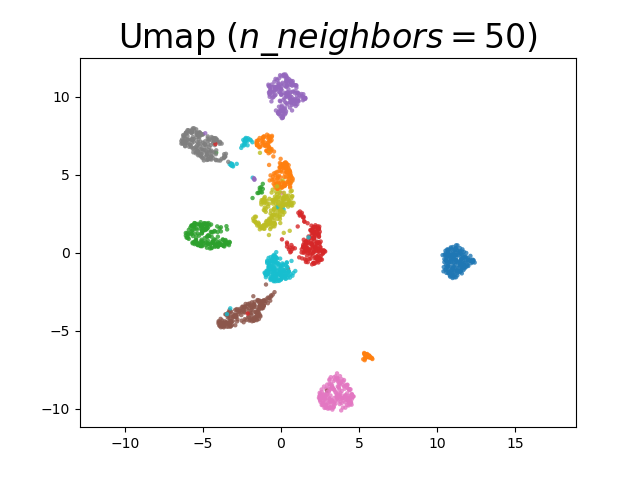
\includegraphics[width=7cm,height=3.5cm\textwidth]{images/umap/umap_digit_n_neighbor_50.png}}
% \subfigure[name2]
{
\label{Fig.sub.2}
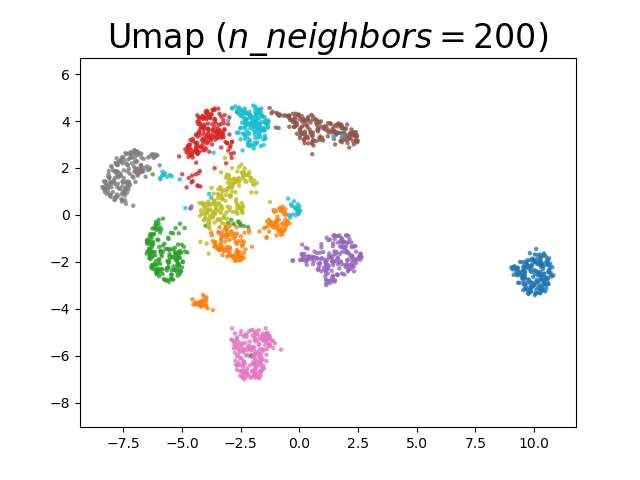
\includegraphics[width=7cm,height=3.5cm\textwidth]{images/umap/umap_digit_n_neighbor_200.png}}
\caption{LD result for UMAP with n\_iter 50 and 200}
% \label{Fig.main}
\end{figure}

\noindent As we can observe from the figure, with the number of $n\_neighbors$ increases, when constructing graphical representations of high-dimensional data, UMAP connects more and more adjacent points, which leads to a projection that more accurately reflects the global structure of the data. When it is a very low value at 2, any idea of global structure has almost completely disappeared. \\

\noindent Different from t-SNE algorithm, UMAP keep more 

% 8/Aug
% 写完umap,开始测largevis的成对变量